\clearpage\section{Results}

{This should include your data analysis and findings}

\begin{figure}[H]
\label{fig:prototype1}
\centering
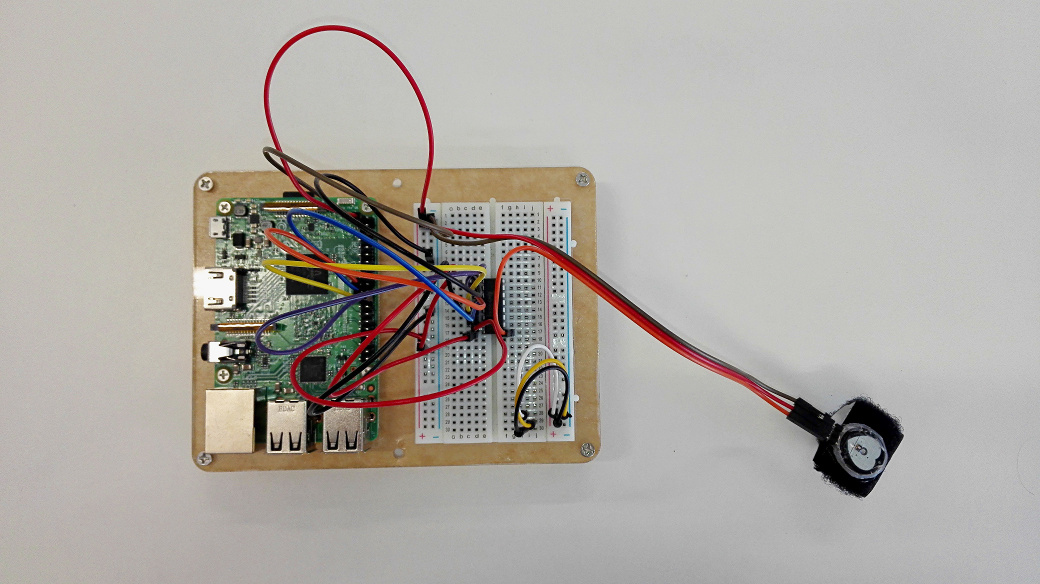
\includegraphics[width=10cm]{img/Chapter4/prototype1_edited.jpg}
\caption[Prototype setup]{\footnotesize{Prototype setup.}}
\end{figure}

\begin{table}[H]
\centering
\caption[This is the caption]{ \footnotesize This is the other caption. Since the trial size of the experiments showed is one second, the number of \textit{Target} and \textit{Impostor} data corresponds to number of trials or seconds}
\label{tab:data_partition}
\footnotesize{
\begin{tabular}{@{}llcccc@{}}
\toprule
\textbf{Dataset}         & \multicolumn{1}{c}{\textbf{Label}} & \textbf{Train} & \textbf{Validation} & \textbf{Develop} & \textbf{Test} \\ \midrule
\midrule
\multirow{3}{*}{First} & Target   & $135$ & $45$  & $30$  & $30$  \\
                         & Impostor & $5,220$    & $1,740$ & $1,890$   & $2,880$    \\
\cmidrule(lr){3-5} \cmidrule(l){6-6}
                         & \#Subjects          & \multicolumn{3}{c}{$31$} & $12$ \\
\midrule
\multirow{3}{*}{Second}  & Target   & $144$ & $80$  & $48$  & $48$  \\
                         & Impostor & $2,014$    & $1,119$    & $1,343$    & $1,545$ \\
\cmidrule(lr){3-5} \cmidrule(l){6-6}
                         & \#Subjects   & \multicolumn{3}{c}{$15$} & $5$ \\ 
\bottomrule
\end{tabular}
}
\end{table}

\begin{algorithm}
\caption{Temperature-Distributed algorithm}\label{alg:tempdistrib}
\begin{algorithmic}[1]
\Procedure{Temp-Spread}{$GN_i, HN_j, temperatures$}\Comment{Lowest temperature priority}
\State $temperature\_list\gets short(temperatures)$
\State $max_temperature\gets max(temperature_list)$
\State $ThresHold\gets 0.5$
\State $temperature\_impact \gets 0.2$
\For{$GN_i$ in $i=1,8$}\Comment{Iterate every hardware node on the given GN}
\State $it\_temperature \gets temperature\_list(GN_i)$
\State $temp\_weight \gets \frac{max\_temperature-it\_temperature}{max\_temperature}*temperature\_impact$
\State $\omega(Master-GN_i) \gets ThresHold*temp\_weight$
\For{$HN_j$ in $j=1,n$}
\If{$available\_accel_{i,j} > busy\_accel_{i,j}$}
    \State $policy_\omega = \frac{Available HW}{Total HW}*ThresHold$
    \State $\omega(GN_i-HN_{i,j}) \gets ThresHold+policy_\omega$
\Else
    \State $\omega(GN_i - HN_{i,j}) \gets 1$
\EndIf

\EndFor
\EndFor
\State $node \gets find\_djistra\_shortest\_path(Master\_Node, aux\_node)$
\State \textbf{$return node$} $b$\Comment{The gcd is b}
\EndProcedure
\end{algorithmic}
\end{algorithm}
